\chapter{Study 1: Classification of music sequencer}
\label{ch: chapter 3}

A big scale study was conducted to create an interface taxonomy of current music sequencer apps on the iOS App Store. In total, 55 music sequencer applications on App Store have been examined (see Appendix \ref{app:Appendix A}). Several search criteria are implemented to locate music sequencer on the App Store (see Section\ref{subsec: search criteria}). After analyzing those music sequencer apps, we proposed classification criteria based on the design of the user interface (see Section \ref{sec: classify criteria}). The 55 music sequencer applications were classify into 3 major groups according to the classification criteria (see Section\ref{sec: result}).

\section{Method}
\label{sec:method}

In total, 71 musical iOS applications associated with music sequencer had been downloaded from App Store. After examined and discussed with my supervisor Ben Swift, 16 applications were removed from the study list either because the application can hardly be classified as music sequencer or because the application was not designed for iPad. The rest 55 music sequencer applications were studied in detailed.

\subsection{Search Criteria}
\label{subsec: search criteria}

Base on \citeauthor{Reference13}'s study which created a whitelisted words for music sequencer, keywords such as \textit{Sequence, Sequencer, Groovebox, Beatbox, Step, MIDI, Pattern, Tempo, BPM, Machine} were used to search on the App Store. Before each application been downloaded, it's description had been briefly overviewed to make sure it was designed for music purpose. Also, in the searching criteria, \textquotedblleft{iPad only}\textquotedblright was chose and results were sorted under the relevance of keywords.

\subsection{Classification criteria}
\label{sec: classify criteria}
The different approaches of interacting with the applications were used to classify the user interface of the music sequencer applications into several categories. The mappings of the sequencer were broke down into 4 operations,
which were \textit{changing pitch, triggering sound, timing and changing timber}.

\textbf{Changing Pitch.} Becasue the way most traditional instruments' pitch were changed discretely, for example, piano, guitar and violin. The majority of musical application including sequencer follow this trend. Besides, pitch is dominated by grid-like, buttom-to-top mapping in music sequencer hardware. Therefore, grid-based, buttome-to-top and discrete pitches layout is widely adopted.

\bigskip
\begin{figure}[h]
  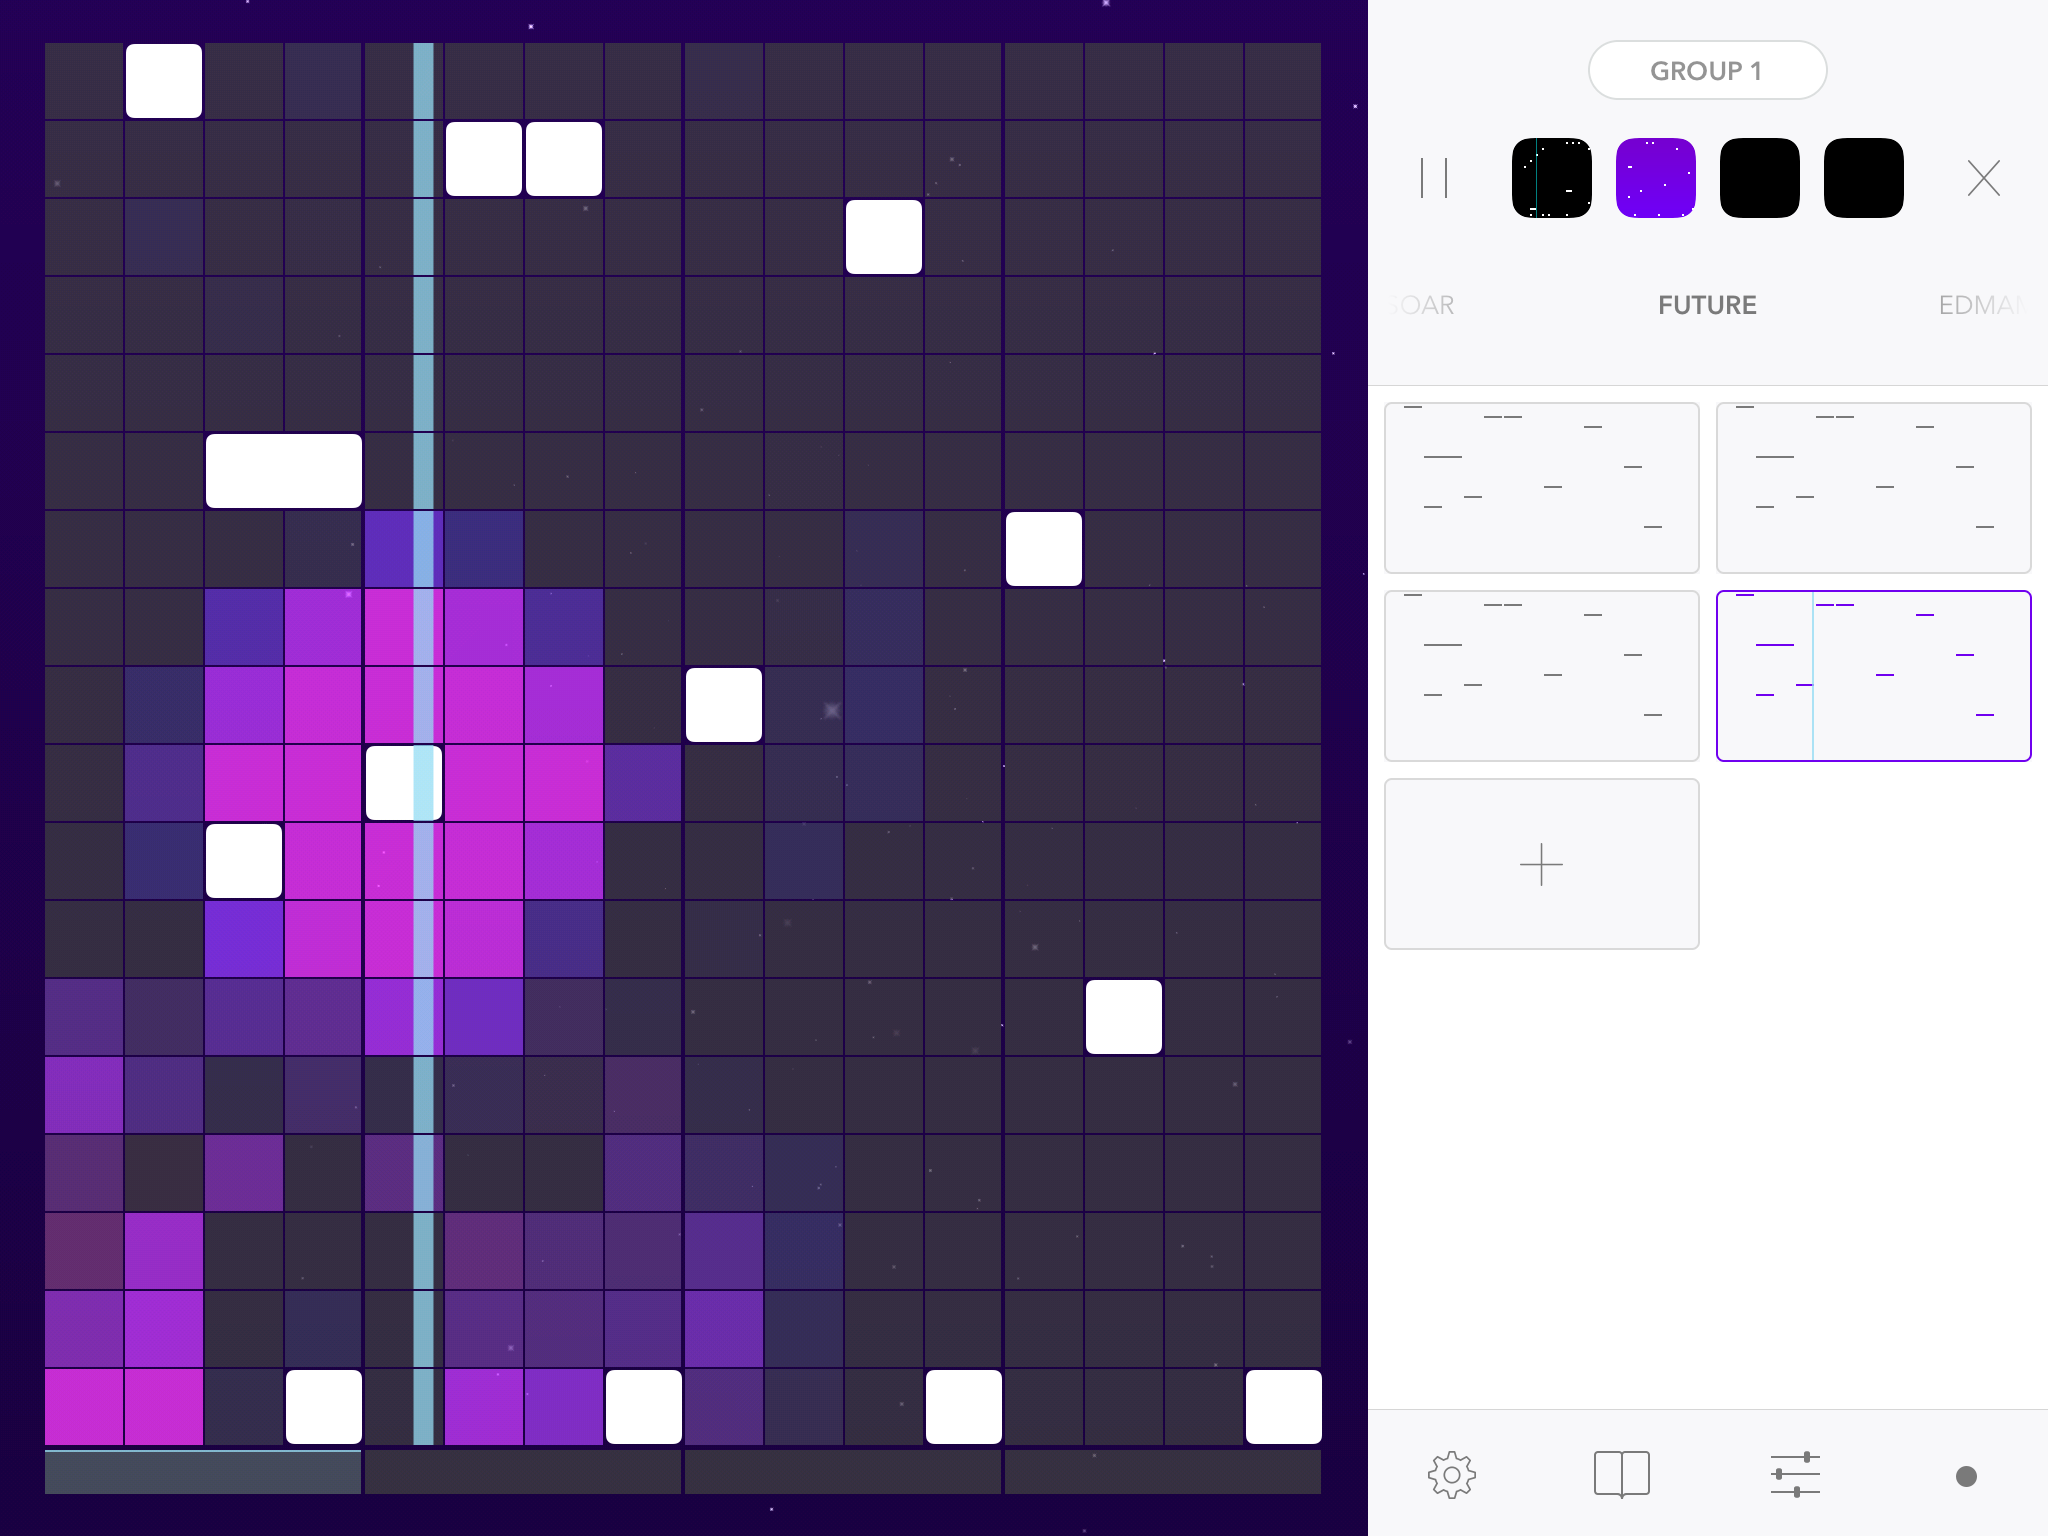
\includegraphics[width=12 cm]{images/Beatwave.PNG}
  \centering
  \caption{Beatwave: grid-based, buttome-to-top and discrete pitch layout}
  \label{fig: Beatwave}
\end{figure}
\bigskip

 Figure \ref{fig: Beatwave} is a good example of this classic interface, in which the interface is divided into 16x16 grids. The time, which is separated into 16 steps, only moves one step at a time from left to right. The blue vertical line works as a reminder of current time, and also indicates what is coming next(in the next step). The white square, on the other hand, represents the sound of a certain instrument. In this case, it represents an electrical sound called \textit{FUTURE}. The column in each step is divided into 16 scales and which are the pitches of the instrument. The white squares located in the top of the grids are high pitch sound of the instrument, on the contrary, the pitch of the sound from the bottom is relatively low.

 \bigskip
 \begin{figure}[h]
   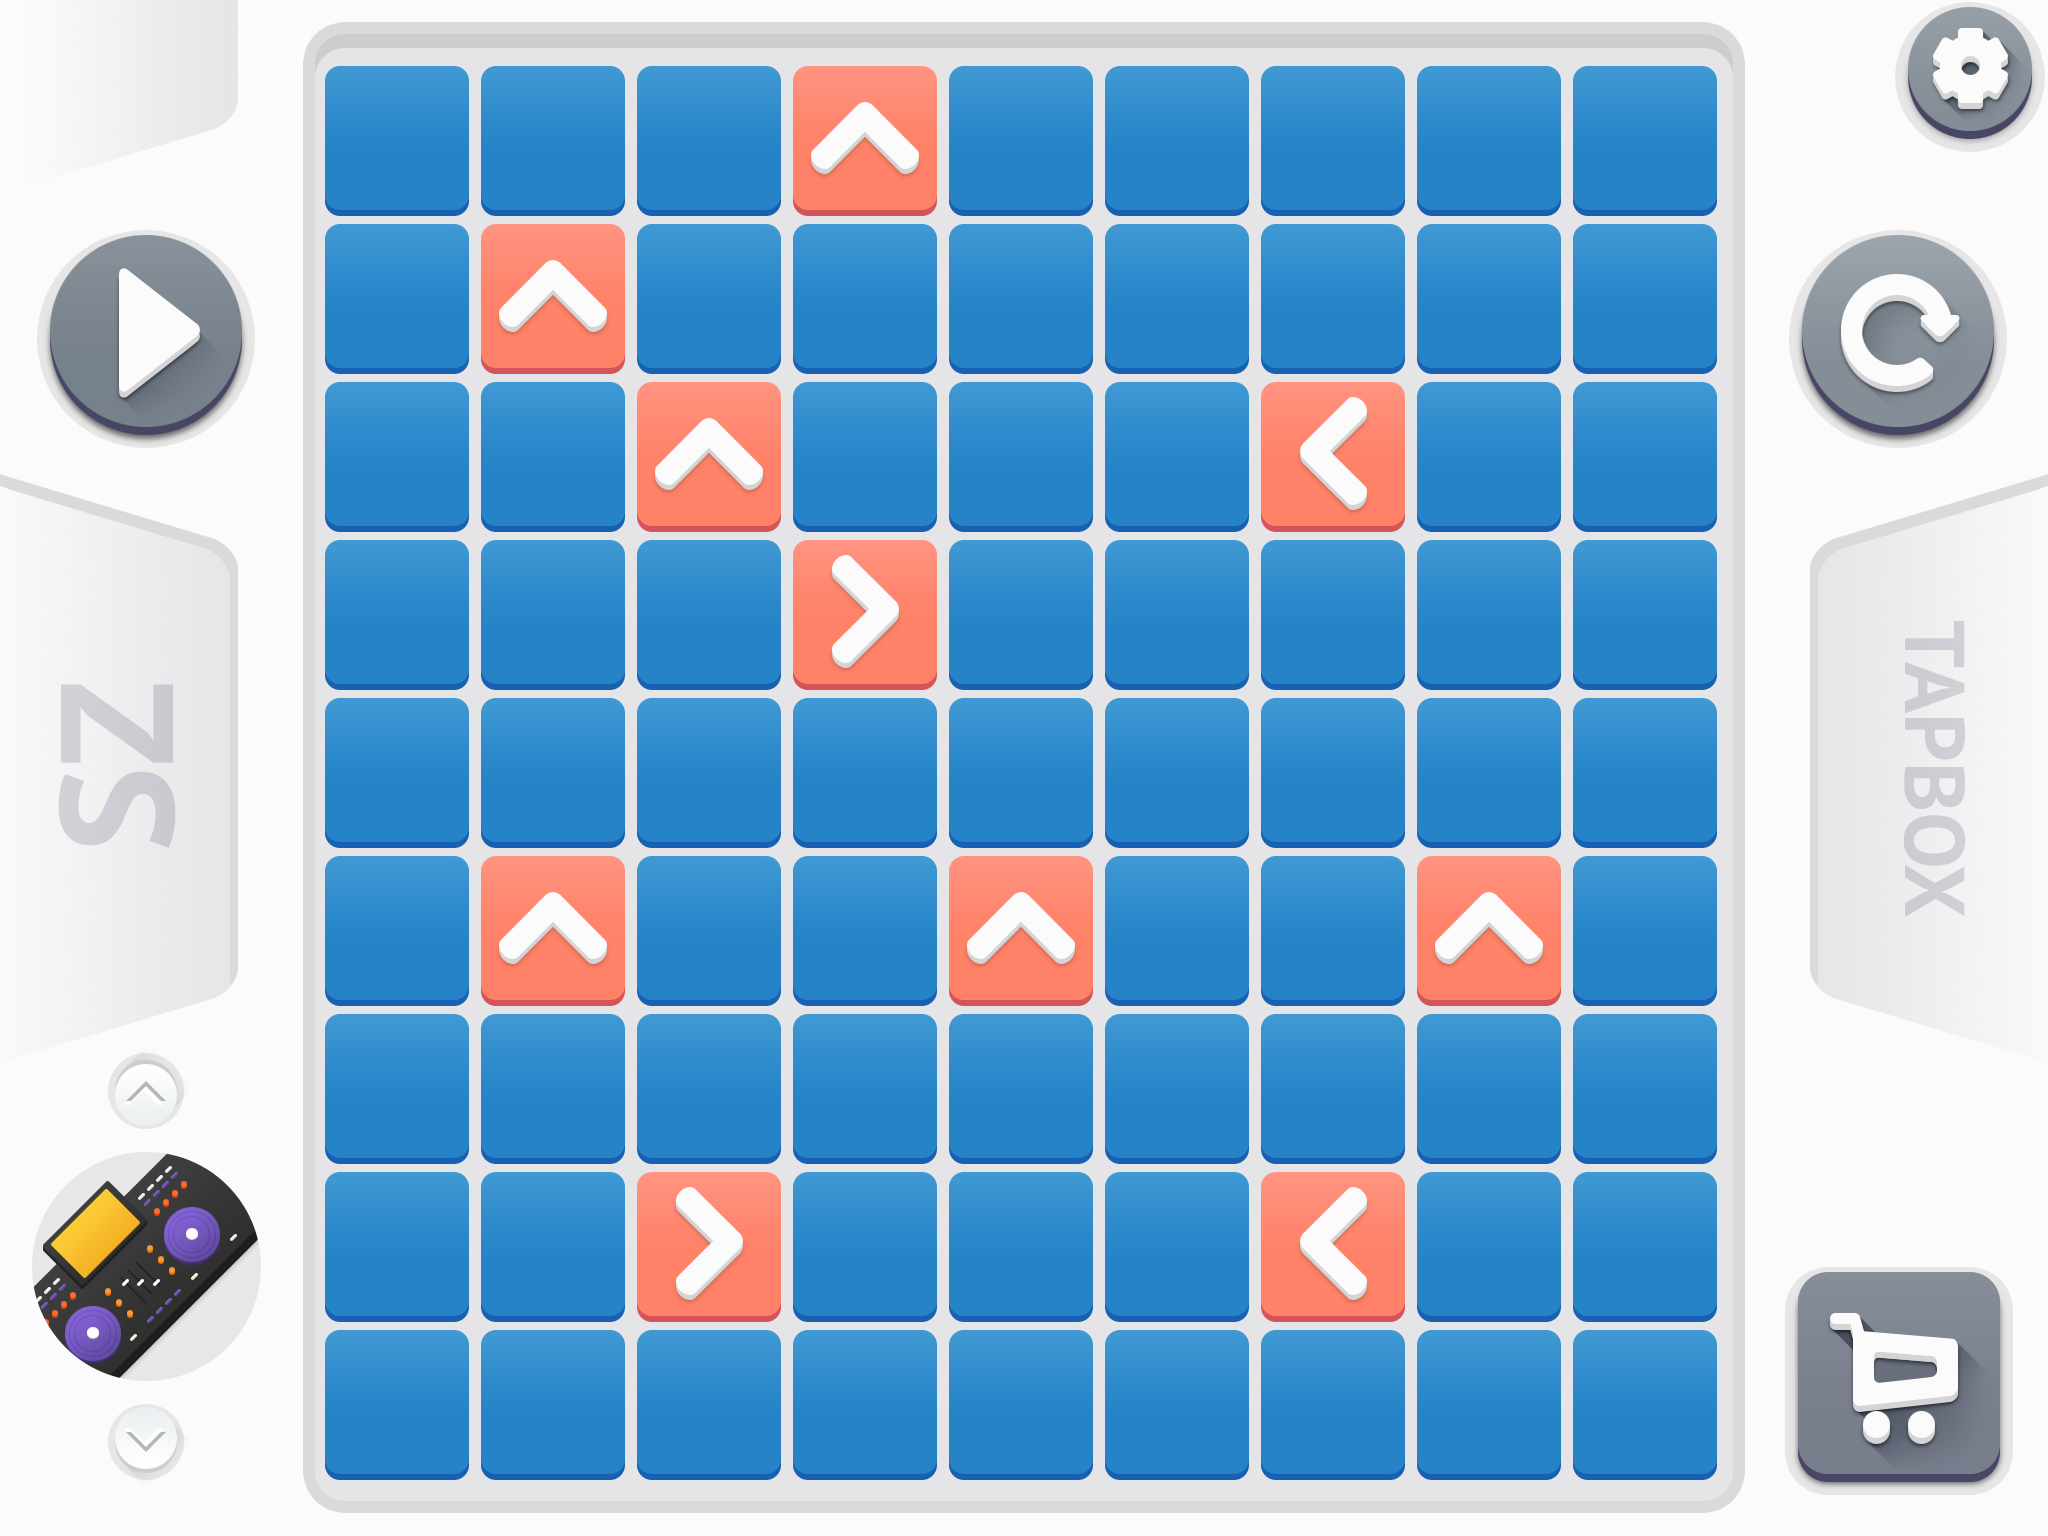
\includegraphics[width=12 cm]{images/SoundZen.PNG}
   \centering
   \caption{SoundZen: grid-based, right-to-left and discrete pitch layout}
   \label{fig: SoundZen}
 \end{figure}
 \bigskip

 However, not all the grid-based sequencer applications increase pitch from bottom to top. There is a small portion of sequencer increase pitch from left to right. For instance, SoundZenHD used a left-to-right pitch mapping (see figure: \ref{fig: SoundZen}).

In addition to the discrete pitch mapping, there are attempts to implement the continuous pitch. \textit{CSketch Lite} followed the classic grid-based layout, but it implements continuous sequencing (see Figure \ref{fig: CSketch}). By implementing the continuous sequenceing, \textit{CSketch Lite} is able to prodecue continuous sound in a series steps rather than make discrete sound step by step, which breaks the bound of the traditional music sequencer. Therefore, the pitch is changing continuously in \textit{CSketch Lite}. In figure \ref{fig: CSketch}, the yellow and blue line denote the trend of pitch changing. Take the top-left yellow line as an example, the pitch of the sound is continuously droping from G$\#$ to F. Even though, the pitch of the above music sequencer applications are still linear mapping.

Except for the linear mapping though the grids, some few Apps adopted the non-linear pitch mapping. For instance, \textit{Orbita} simulates the movemment of a small planet orbits around a central planet along an elliptical path. And in this case, different color of \textquotedblleft{planet}\textquotedblright represent different instruments, which produces sound while elliptical orbit. The pitch is changing continuously based on the distance between the small planet and the central planet(see figure \ref{fig: Orbita}).

\begin{figure}
  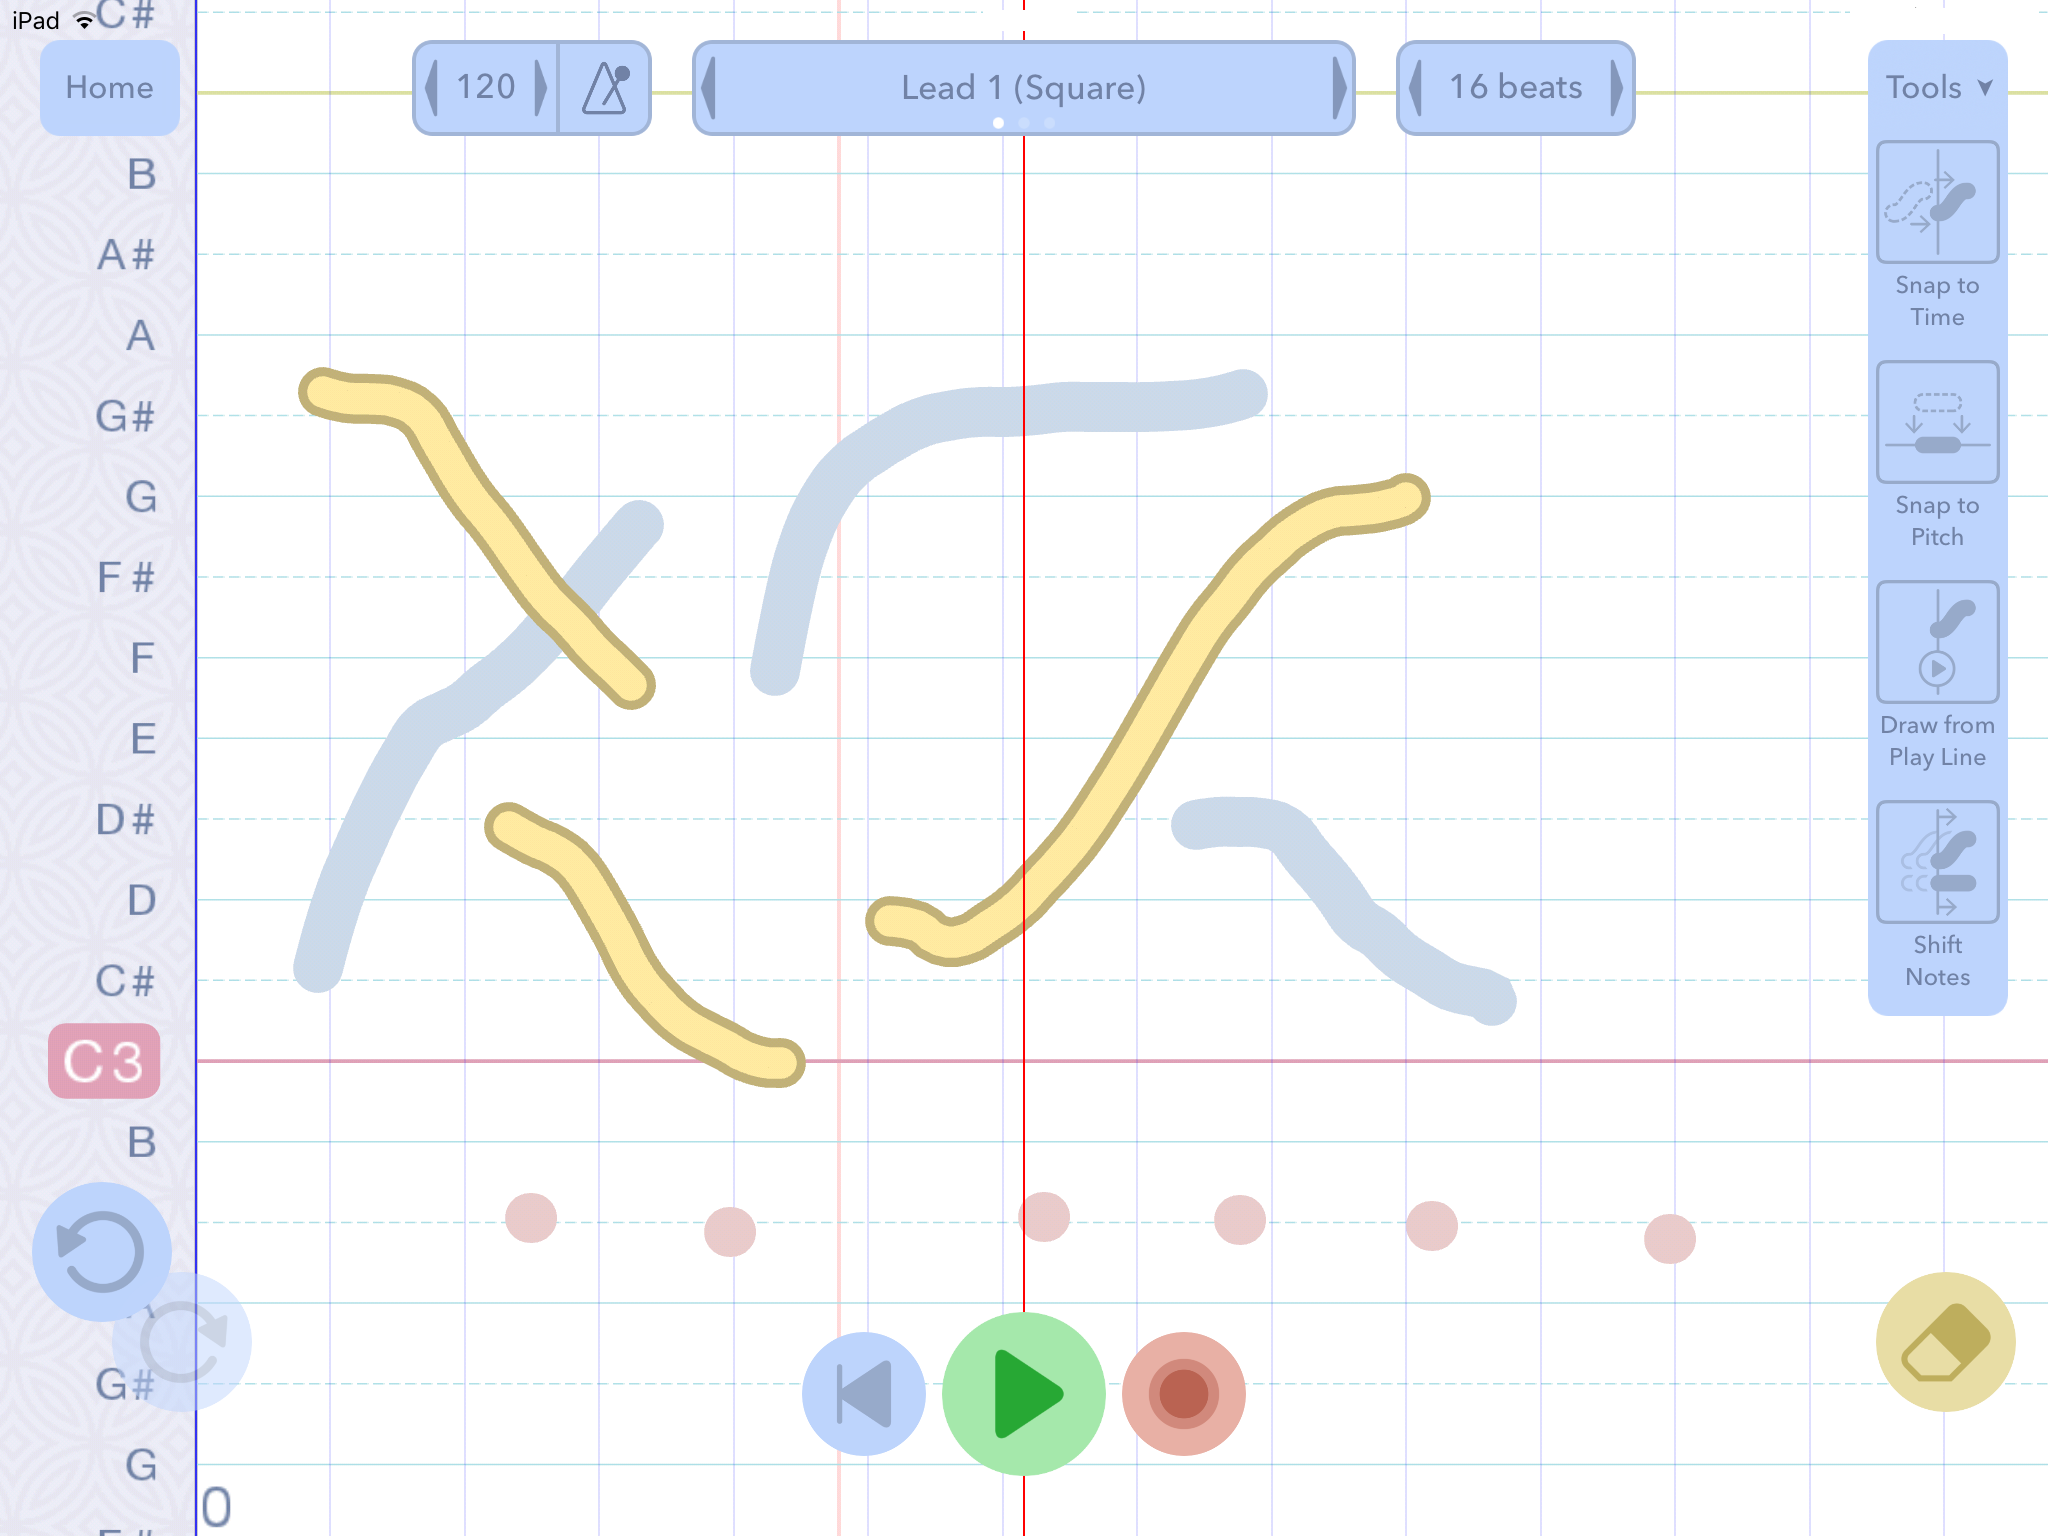
\includegraphics[width=12 cm]{images/CSketch_Lite.PNG}
  \centering
  \caption{CSketch Lite: grid-based, top-to-bottom and continuous pitch layout}
  \label{fig: CSketch}
\end{figure}

It is not unusal of mapping pitch to colour in music applications \citep{Reference14}. However, there was only one music sequencer found to represent pitch with different colors.  

\newpage
\bigskip
\begin{figure}
  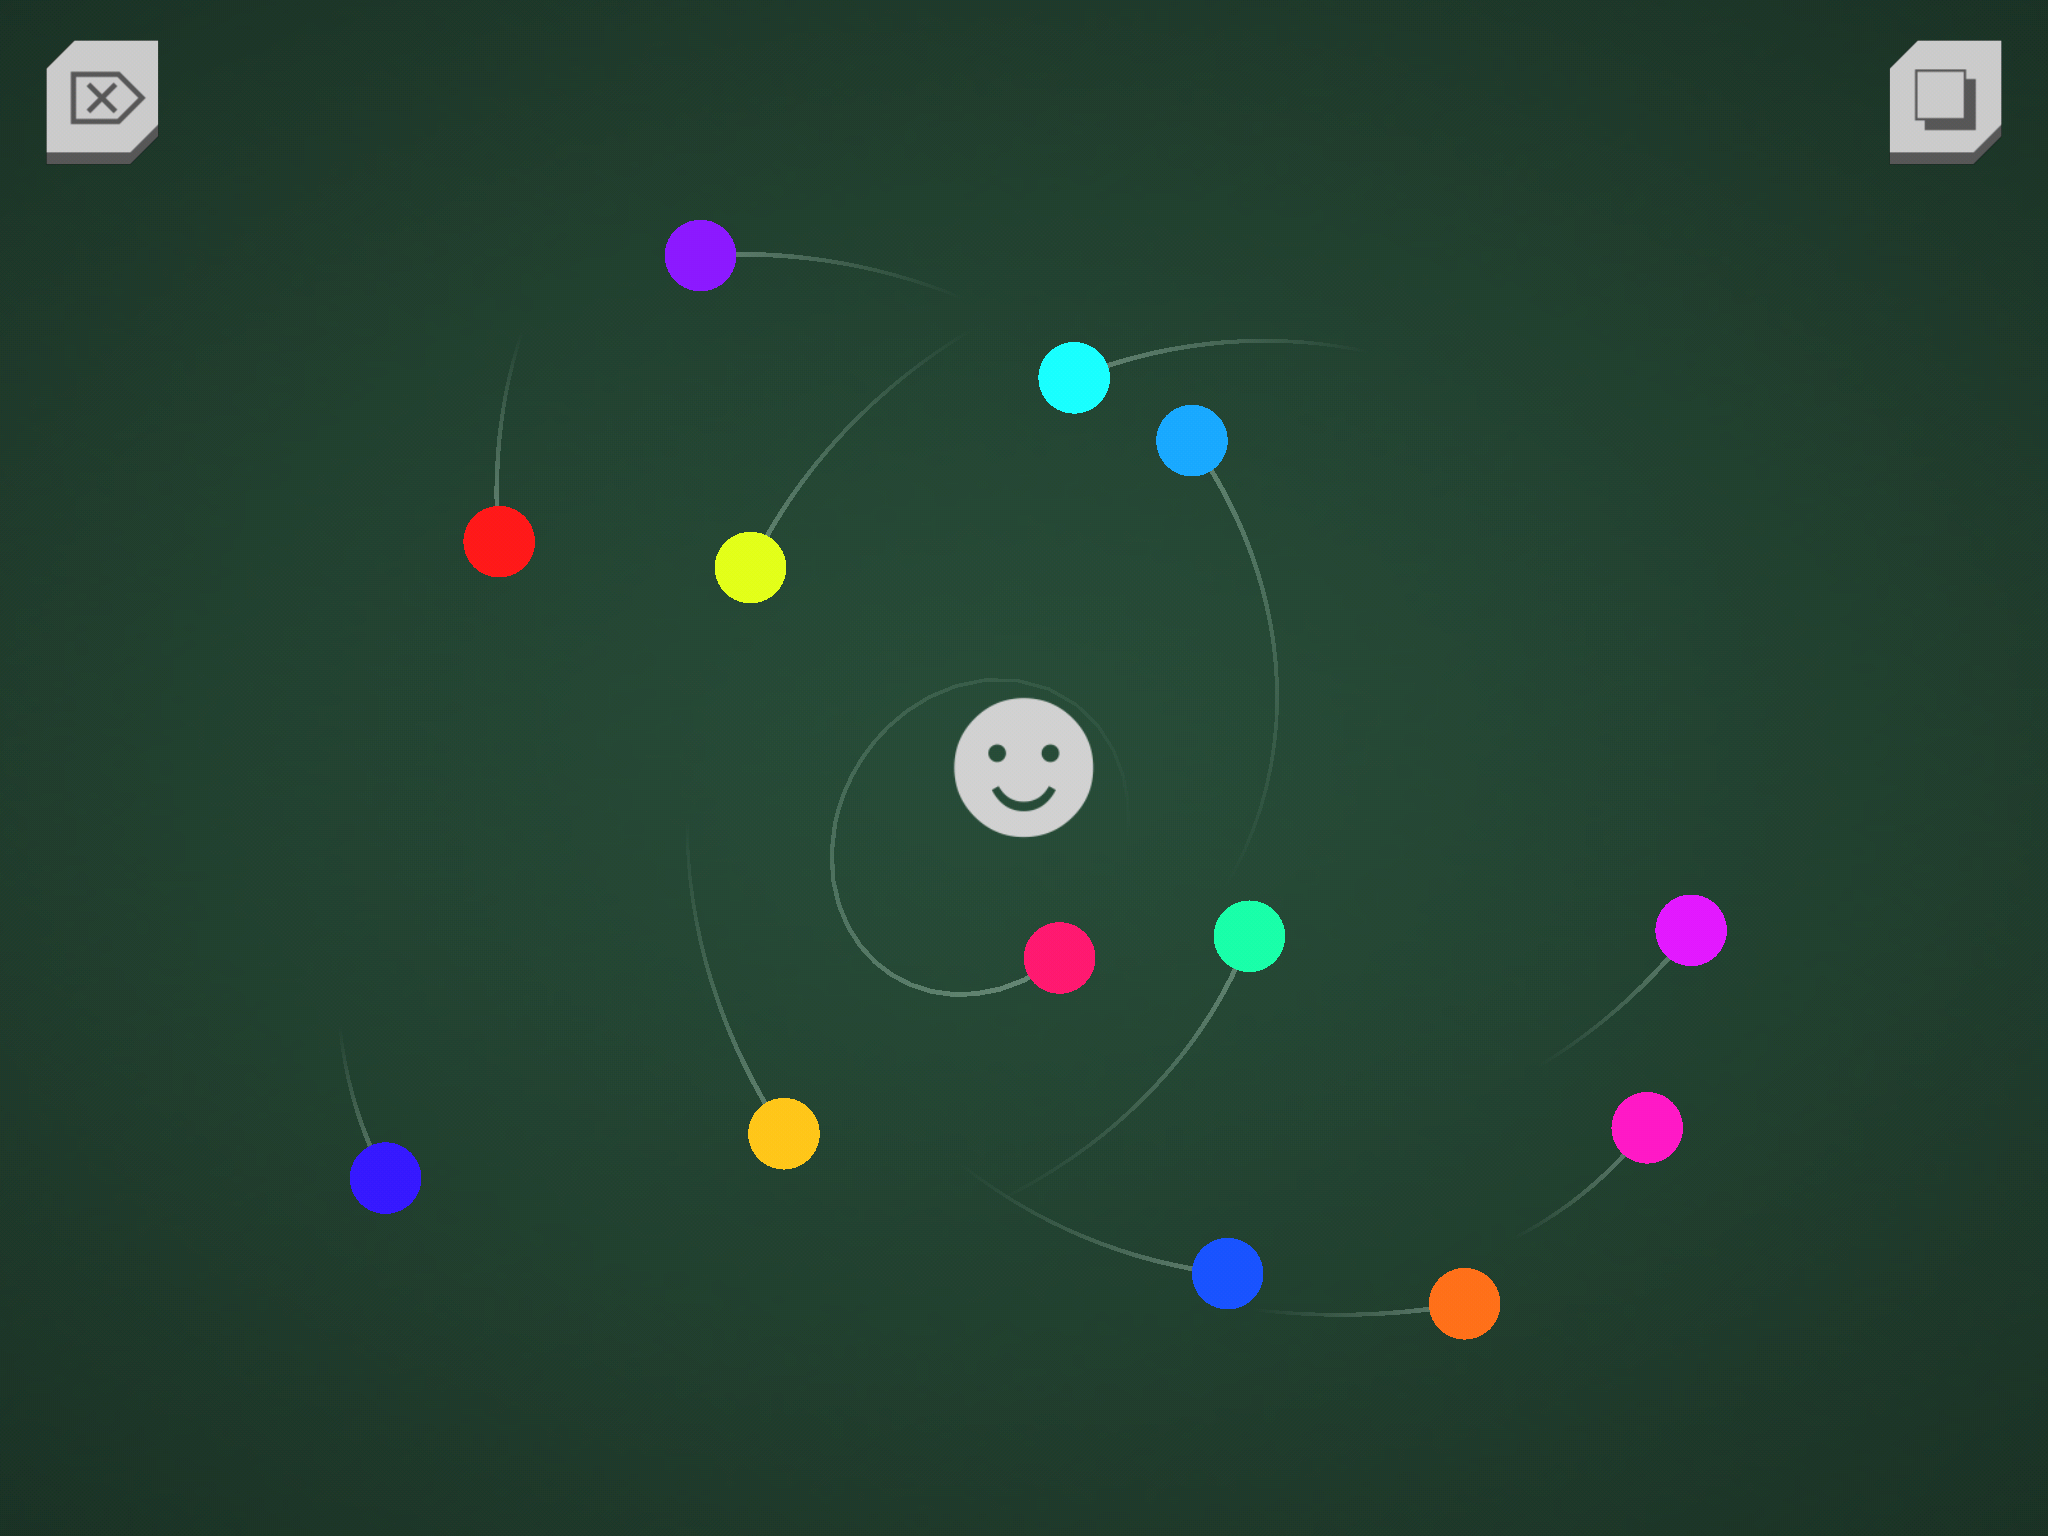
\includegraphics[width=12 cm]{images/Orbita.PNG}
  \centering
  \caption{Orbita: elliptical orbita, non-linear and continuous pitch layout}
  \label{fig: Orbita}
\end{figure}
\bigskip

\section{Results}
\label{sec: result}
